\subsection{Conceptual model and assumptions}
\noindent The goal of this academic project is to apply the concept of Agent Based Modelling and system thinking to explore the trade-offs in the policy space of the municipality to optimize the plastic recycling rate. To do this, two research approaches will be employed. First, an exploratory model approach to answer the 1st research question presented in the introduction. Second, a hypothesis-driven approach to address the second above-mentioned question. 

\subsubsection{System and agents}
\noindent The analysed socio-technical system is a Dutch plastic recycling system organised at the municipality level. The project investigates interactions between three central agents in the municipality of Delft: households, municipality and the recycling companies. \\

\underline{Households:}\\
\noindent In this system, households generate waste from daily life consumption. The volume produced on a daily basis depends on the typology of the household. The following four types are ordered according to the quantity of waste produced, from the least to the most producing: elderly, single, couple and family. \\

\begin{table}[h]
\centering
\caption{Background information about Delft municipality}
\begin{tabular}{cc}
\rowcolor[HTML]{666666} 
{\color[HTML]{FFFFFF} Characteristic}                             & {\color[HTML]{FFFFFF} \textbf{Data}} \\
Delft population                                                  & 103 581 inhabitants                  \\
Average household size                                            & 2.15 people                          \\
Number of households                                              & 48 177                               \\
Average yearly waste production per capita (Zuid-Holland) in 2020 & 491 kg                               \\
Average yearly plastic production per capita (NL) in 2020         & 96 kg                               
\end{tabular}
\end{table}\\

\begin{table}[h]
\centering
\caption{Representation of household types in the population}
\begin{tabular}{ccc}
\rowcolor[HTML]{666666} 
{\color[HTML]{FFFFFF} \textbf{Household}} & {\color[HTML]{FFFFFF} \textbf{Percentage}} & {\color[HTML]{FFFFFF} \textbf{Number of inhabitants}} \\
Single elderly household (65+)            & 4\%                                        & 4 143                                                 \\
Couple elderly household (65+)            & 12\%                                       & 12 430                                                \\
Single                                    & 60\%                                       & 62 149                                                \\
Couple                                    & 17\%                                       & 16 380                                                \\
Family                                    & 7\%                                        & 8 479                                                
\end{tabular}
\end{table}

\noindent The average quantity of waste produced depends on the type of household and the number of people living in the household. General waste and plastic production in table XY belong to the reference case of a single household (i.e. per capita). For elderly, we assume they produce 20 percent less waste than a single household due to a smaller consumption. Couple household generates twice as much trash than a single household. Finally, based on the number of households and the percentage of family households in Delft municipality, the model will assume that the average family size is 2.5 people. Therefore, a family household produces 2.5 times more waste than a single household. It is important to note that the share of plastic production versus total waste production remains the same across all household types.\\

\noindent In Delft, households are responsible for the 1st sorting phase of the recycling process. At home, plastics should be separated from other types of trash. Then, citizens are provided with collection containers in their neighborhood for throwing waste away and allowing the municipality to start the collection process. In addition, some neighbourhoods benefit from "at home collection" consisting of a second collection channel. The “purity” of plastic trash, which is the percentage of plastics in plastic bins (supposed to be 100 percent), is directly influenced by three factors: perception, importance and knowledge of recycling. In this model, it is assumed that the three factors do not affect each other. \\

\begin{figure}[H]
    \centering
        \captionsetup{width=\linewidth}
        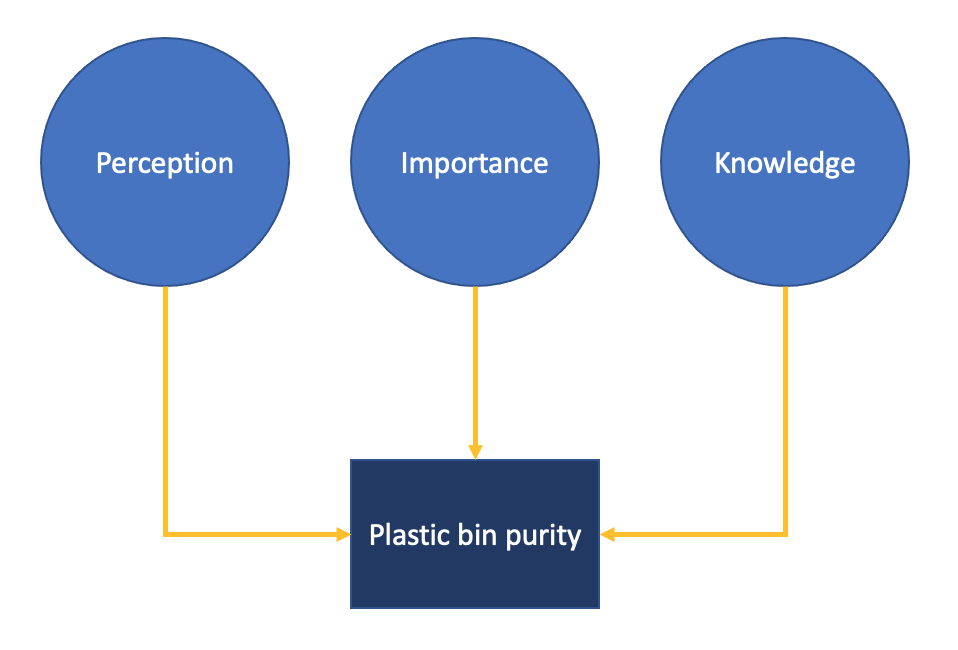
\includegraphics[width=0.7\linewidth]{Images/influences.png}
        \caption{Relationship between perception, importance, knowledge and plastic bin purity.}
    \label{fig:Relationship between perception, importance, knowledge and plastic bin purity.}
\end{figure}

\underline{Municipality:}\\
\noindent The municipality of Delft is responsible for providing the collection containers to households, collecting waste across the neighbourhoods from the containers and transferring the trash to the recycling facilities. To fulfill these obligations, the municipality contracts a waste collection company. \\

\noindent Currently the municipality collects XXX tonnes of waste on a daily basis and recycles XX\%. The municipality targets a recycling rate of XX\%, XX\% and XX\% respectively by 2030, 2035 and 2040. \\

\underline{Recycling company:}\\
After being transferred by the collection company to the recycling company, waste enters the recycling process that is made of three phases. The first phase is sorting where plastics are separated from non-plastic waste. The second phase is washing and flaking where plastics are cleaned and shredded in small pieces. The third step is regranulating and  compounding. During this phase, shredded plastic is transformed in granules and then compressed in blocks. As you can see in figure XY, the scope of the model starts with the production of waste production and ends with regranulating and compounding. After being separated from plastic waste, non-plastic waste is not further investigated. The same goes for plastic not suitable for recycling and plastic loss incurred during the recycling process. \\

\begin{figure}[H]
    \centering
        \captionsetup{width=\linewidth}
        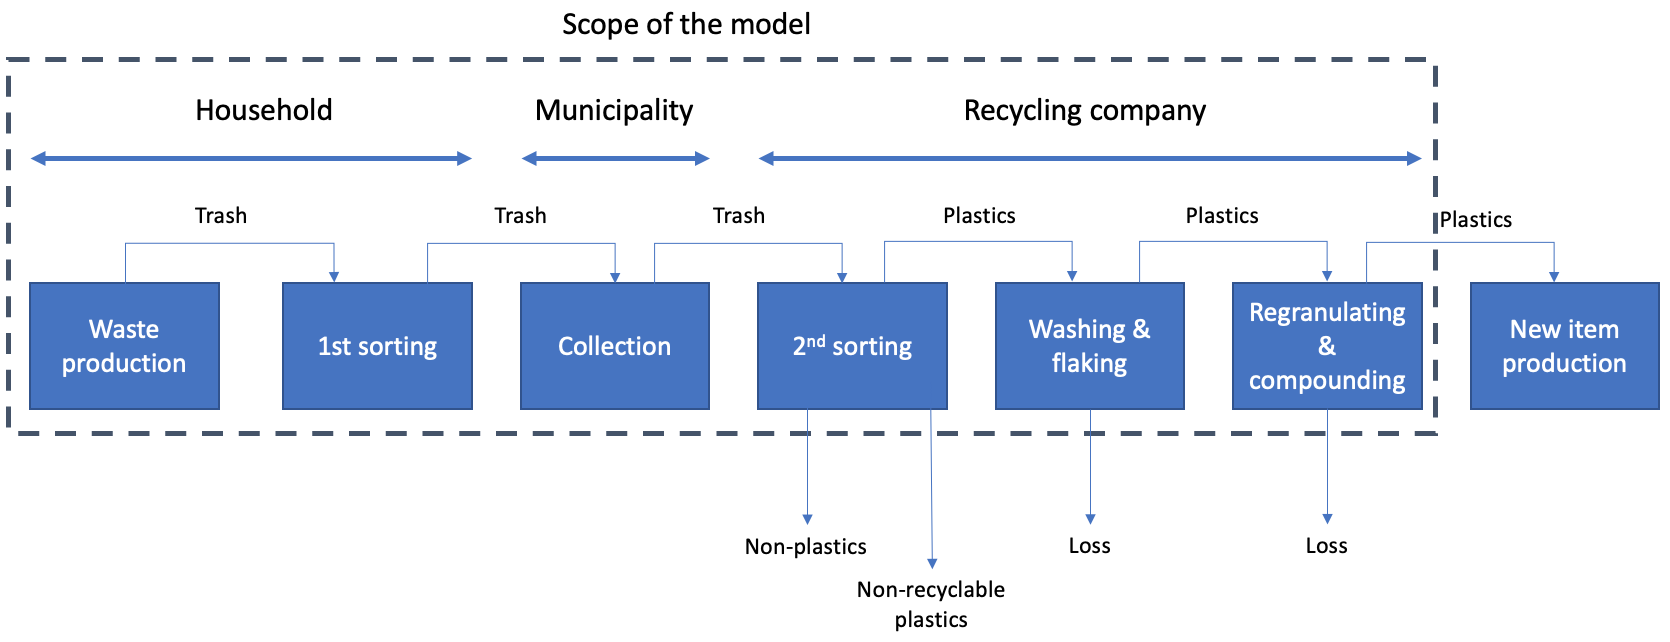
\includegraphics[width=1\linewidth]{Images/model scope.png}
        \caption{Scope of the recycling model.}
    \label{fig:Scope of the recycling model.}
\end{figure}\\

\subsection{Use Case Diagram}
\noindent In this sub chapter the model as described above is visually illustrated in a Use Case Diagram in figure \ref{fig:Use_Case}.

\begin{figure}[H]
    \centering
        \captionsetup{width=\linewidth}
        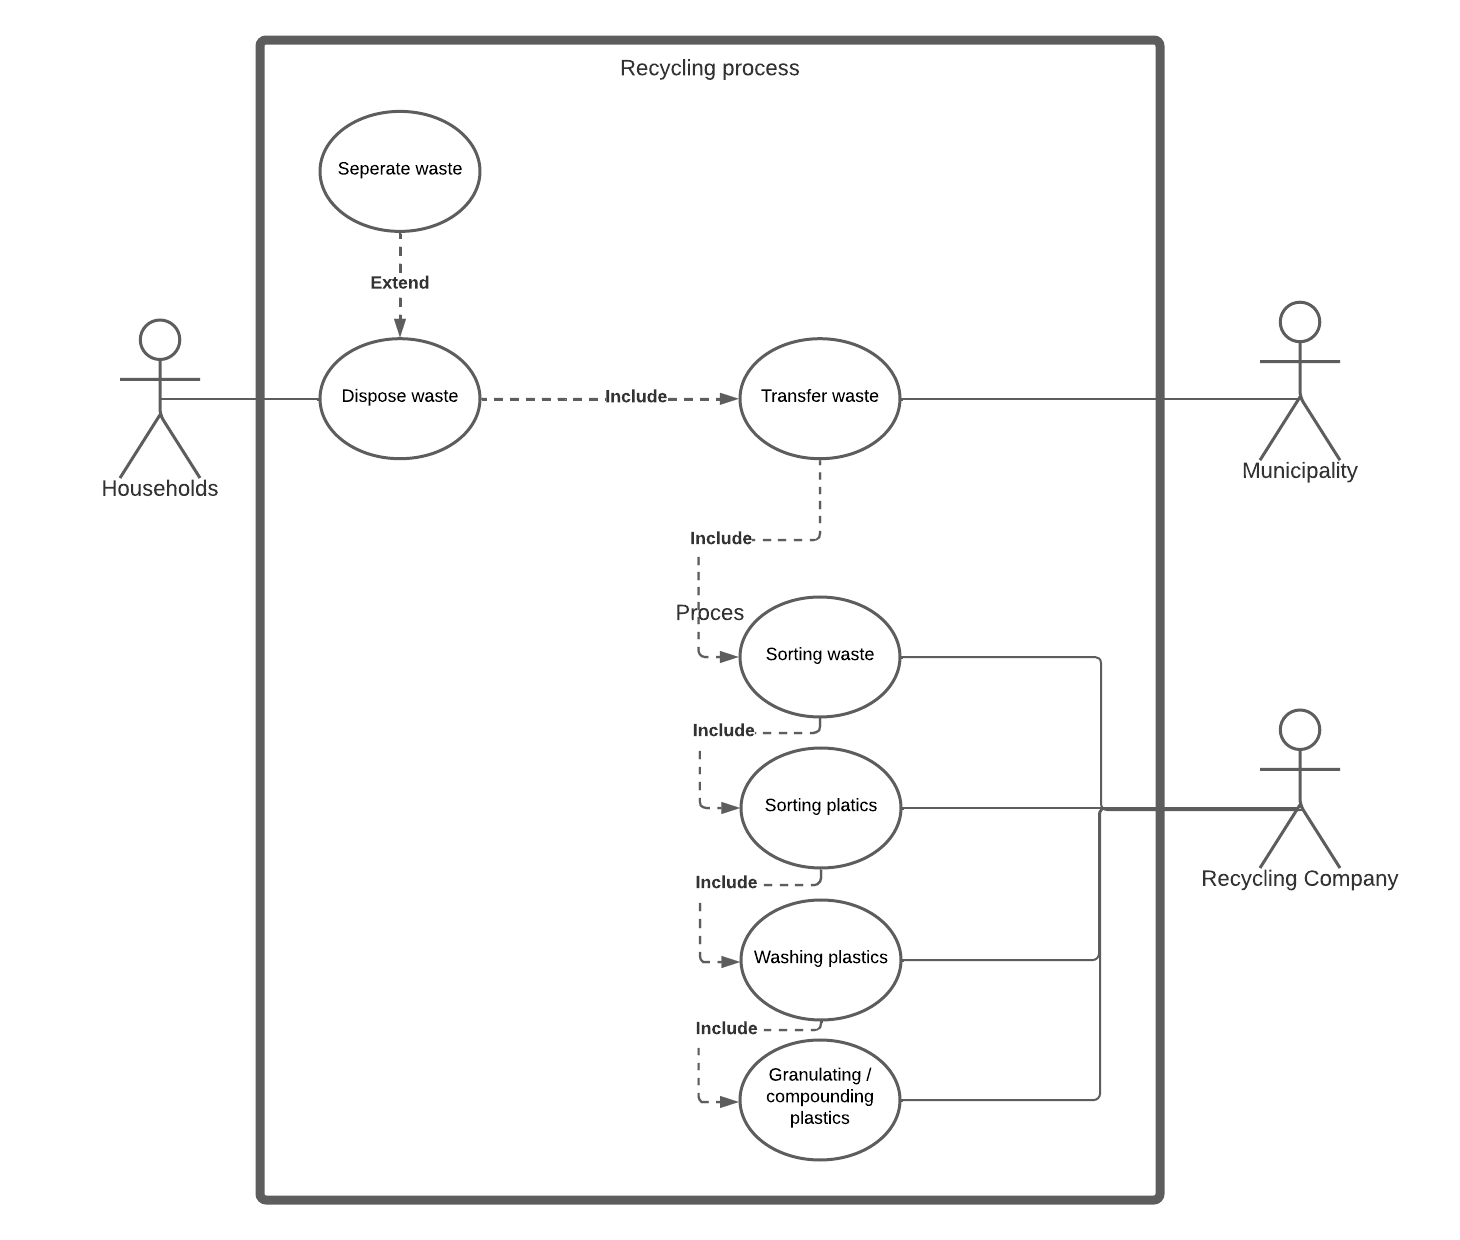
\includegraphics[width=1\linewidth]{Images/UML for recycling system - Use case.png}
        \caption{Use Case Diagram waste recycling process)}
    \label{fig:Use_Case}
\end{figure}

\noindent The process starts with the households. They will deposit their waste at containers located in the neighborhood. The trash is produced at home ,sorted at home and brought to the container. Households may also not follow the sorting rules, and not separate the waste. Therefore Separation waste' is an extend of the 'Deposit waste'. 

\noindent The next entity is the municipality. Their use case is to transfer the waste from the containers to the recycling company. In order to transfer waste, the waste must have been deposit in the container. Due to this reason the 'Deposit waste' must be included by the 'Transfer waste' use case.

\noindent The third entity is the Recycling company. Their first use case is to sort plastic waste from non-plastic waste. In order to do that, the waste must be present, wherefore the 'Transfer waste' use case is included in the 'Sorting waste' use case. The sorting process which follows after the sorting are all have included relations. That is due to the fact that these steps needs to be full filled all individually before the next step can start. 

